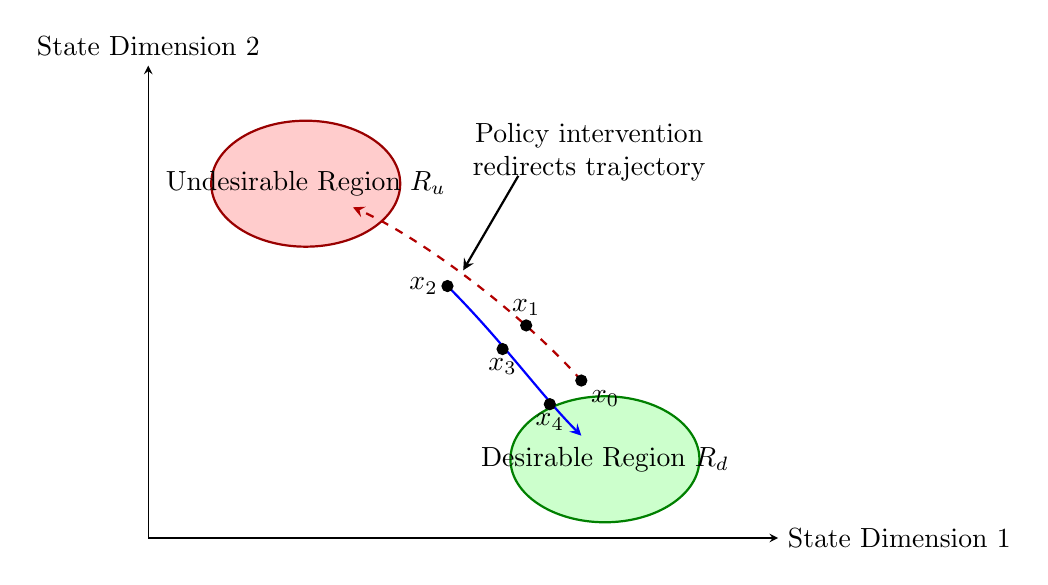
\begin{tikzpicture}[scale=1.0, >=stealth]

% Axes
\draw[->] (0,0) -- (8,0) node[right] {State Dimension 1};
\draw[->] (0,0) -- (0,6) node[above] {State Dimension 2};

% Desirable region
\filldraw[fill=green!20, draw=green!50!black, thick] (5.8,1.0) ellipse (1.2 and 0.8);
\node at (5.8,1.0) {Desirable Region $R_d$};

% Undesirable region
\filldraw[fill=red!20, draw=red!60!black, thick] (2.0,4.5) ellipse (1.2 and 0.8);
\node at (2.0,4.5) {Undesirable Region $R_u$};

% Initial trajectory (drifting toward instability)
\draw[thick, dashed, red!70!black, ->] 
(5.5,2.0) .. controls (4.8,2.8) and (3.5,3.8) .. (2.6,4.2);

% Corrected trajectory (policy intervention)
\draw[thick, blue, ->] 
(3.8,3.2) .. controls (4.5,2.5) and (5.0,1.8) .. (5.5,1.3);

% State points
\filldraw[black] (5.5,2.0) circle (2pt) node[below right] {$x_0$};
\filldraw[black] (4.8,2.7) circle (2pt) node[above] {$x_1$};
\filldraw[black] (3.8,3.2) circle (2pt) node[left] {$x_2$};
\filldraw[black] (4.5,2.4) circle (2pt) node[below] {$x_3$};
\filldraw[black] (5.1,1.7) circle (2pt) node[below] {$x_4$};

% Policy intervention label
\draw[->, thick] (4.7,4.6) -- (4.0,3.4);
\node[align=center] at (5.6,4.9) {Policy intervention\\redirects trajectory};

\end{tikzpicture}
